%! Author = Len Washington III
%! Date = 9/19/2023

% Preamble
\documentclass[12pt]{report}

% Packages
\usepackage[10]{cs430lecture}

% Document
\begin{document}

%<*Lecture-Activity-10>
\newcommand{\bsttree}{\tikzset{every tree node/.style={minimum width=2em,draw,circle},
         blank/.style={draw=none},
         edge from parent/.style=
         {draw,edge from parent path={(\tikzparentnode) -- (\tikzchildnode)}},
         level distance=1cm}
			\begin{tikzpicture}
			\Tree
			[.$15$
				[.$6$
					[.$3$
						[.$2$ ]
						[.$4$ ]
					]
					[.$7$
						[.$13$
							[.$9$ ]
						]
					]
				]
				[.$18$
					[.$17$ ]
					[.$20$ ]
			]]
			\end{tikzpicture}}
\section{Opening Questions}\label{sec:opening-questions-10}
\begin{enumerate}[label=\arabic*.]
    \item In your own words explain how you insert a new key in a binary search tree. \answer{When you have a value, you compare the value you're inserting to the value in the node. If the inserting value is less than the value, you recursively call the Insert function with the left node. If the value was greater, you recursively call Insert on the right node.}
	\item Give an example of a series of 5 keys inserted one at a time into a binary search tree that will yield a tree of height 5.\answer{\\\tikzset{every tree node/.style={minimum width=2em},
         blank/.style={draw=none},
         edge from parent/.style=
         {draw,edge from parent path={(\tikzparentnode) -- (\tikzchildnode)}},
         level distance=1cm}
	\begin{tikzpicture}
		\Tree
		[.$5$
			[.$7$
				[.$9$
					[.$8$
						[.$8.5$ ]
					]
				]
		]]
		\end{tikzpicture} The runtime of Insert is $O(h)$ where $h$ is the height of the tree.}
	\item If we do a left rotate on node $X$ below, explain which left and/or right child links need to be changed.\\
\tikzset{every tree node/.style={minimum width=2em},
         blank/.style={draw=none},
         edge from parent/.style=
         {draw,edge from parent path={(\tikzparentnode) -- (\tikzchildnode)}},
         level distance=1cm}
	\begin{tikzpicture}
		\Tree
		[.$X$
			[.$a$ ]
			[.$Y$
				[.$b$ ]
				[.$c$ ]
		]]
		\end{tikzpicture}\answer{\begin{tikzpicture}
		\Tree
		[.$Y$
			[.$X$
				[.$a$ ]
				[.$b$ ]
			]
			[.$c$ ]
		]
		\end{tikzpicture} This tree maintains the relationships of the first tree. $c$ was already larger than $Y$, which is maintained. $b$ was smaller than $Y$ but larger than $X$, which has also been maintained. But now the height of $C$ has been decreased by 1.}
\end{enumerate}

\section{Tree depth vs Tree Height}\label{sec:tree-depth-vs-tree-height}
The length of the path from the root $r$ to a node $x$ is the depth of $x$ in $T$. The height of a node in a tree is the number of edges on the longest simple downward path from the node to a leaf, and the height of a tree is the height of its root. The height of a tree is also equal to the largest depth of any node in the tree.
\begin{figure}[H]
	\centering
	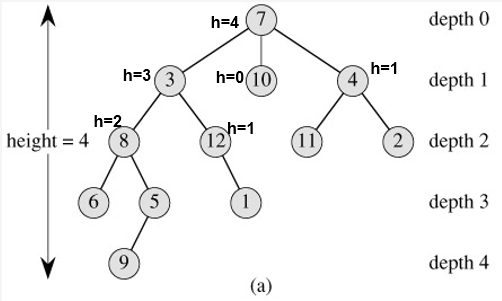
\includegraphics[width=\textwidth]{10.1}
	\caption{Height vs Depth of a Tree}
	\label{fig:tree-height-depth}
\end{figure}

\section{BST Operations}\label{sec:bst-operations}
\begin{enumerate}[label=\arabic*)]
    \item Write pseudocode for BST Successor \answer{(next larger value)} (or Predecessor). Demonstrate on the below tree from node 15 and then node 13.\\\bsttree\\\answer{\begin{algorithm}[H]
    		\caption{Binary Search Tree Successor (Best: $O(1)$, Worst: $O(h)$)}\label{alg:bst-successor}
    		\begin{algorithmic}[1]
    		\Function{Successor}{$p$: Node}\Comment{The Successor is usually the min of the graph in the right node, essentially, right than left-left-$\dots$-left.}
				\If{$p.right$ exists}
					\State \Return \Call{Min}{$p.right$}
				\Else
					\State go up until you go up on left pointer
					\If{never go up left}
						\State \Return null \Comment{You started in the largest value.}
					\EndIf
				\EndIf
    		\EndFunction
    		\end{algorithmic}
    	\end{algorithm}}
	\item Write pseudocode for BST Insert. Demonstrate on the below tree to insert 5 and then 19.\\\bsttree\\\answer{\begin{algorithm}[H]
			\caption{Binary Search Tree Insert ($O(h)$)}\label{alg:bst-insert}
			\begin{algorithmic}[1]
			\Function{Insert}{$key$}
				\If{$root == $ null}
					\State $root \gets$ \Call{Node}{$key$}
					\State \Return
				\EndIf
				\State $p \gets$ $root$
				\State $q \gets$ null\Comment{Following the parent node}
				\While{$p \neq $ null}
					\If{$p.val > key$}
						\State $q\gets$ $p$
						\State $p\gets p.left$ \Comment{Go Left}
					\Else
						\State $q\gets$ $p$
						\State $p\gets p.right$ \Comment{Go Right}
					\EndIf
				\EndWhile
				\If{$q.val > key$}
					\State $q.left \gets $ \Call{Node}{$key$}
				\Else
					\State $q.right \gets$ \Call{Node}{$key$}
				\EndIf
			\EndFunction
			\end{algorithmic}
		\end{algorithm}}
	\item What are the three possible cases when deleting a node from a BST?\\\bsttree\\\answer{\begin{itemize}
		\item No children
		\begin{itemize}
			\item Set the $parent.left$ or $parent.right$ (depending on where you came from) to null; $O(1)$.
		\end{itemize}
		\item One child
		\begin{itemize}
			\item Make the parent of the child point to the child of the node you're deleting (essentially splicing out the node you're deleting); $O(1)$.
		\end{itemize}
		\item Two children
		\begin{itemize}
			\item Swap the predecessor or successor value into the node, and then deleting the value where the predecessor|successor was.\begin{algorithm}[H]
					\caption{Delete A Node with 2 Children from a BST}\label{alg:bst-delete-2-children}
					\begin{algorithmic}[1]
					\Function{Delete2Child}{$p$: Node}
						\State $successor \gets$ \Call{\hyperref[alg:bst-successor]{Successor}}{$p$} \Comment{Or Predeccesor, $O(h)$}
						\State $p.value \gets$ $successor.value$\Comment{$O(1)$}
						\State \Call{\hyperref[alg:bst-delete]{Delete}}{$successor$}\Comment{$O(h)$}
					\EndFunction
					\end{algorithmic}
				\end{algorithm}
		\end{itemize}
	\end{itemize}}
	\item Write pseudocode for BST Delete (assume you already have a pointer to the node)\answer{\begin{algorithm}[H]
			\caption{Binary Search Tree Delete}\label{alg:bst-delete}
			\begin{algorithmic}[1]
			\Function{Delete}{$p$: Node}\Comment{}
				\State
			\EndFunction
			\end{algorithmic}
		\end{algorithm}}
\end{enumerate}

\section{BST Rotations}\label{sec:bst-rotations}
Local operation in a search tree that maintains the BST property and possibly alters the height of the BST.\\

$x$ and $y$ are nodes; $a$, $b$, $c$ are sub trees
\begin{figure}[H]
	\centering
	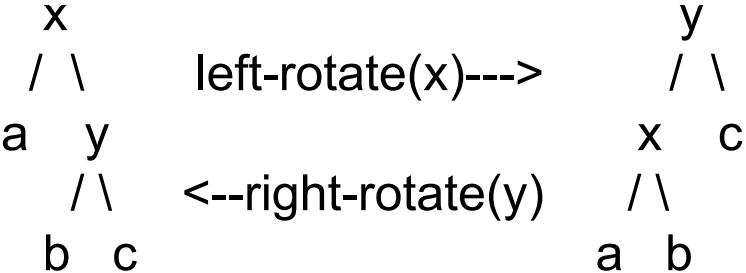
\includegraphics[width=\textwidth]{10.tmp}
	\label{fig:}
\end{figure}

%\tikzset{every tree node/.style={minimum width=2em},
%         blank/.style={draw=none},
%         edge from parent/.style=
%         {draw,edge from parent path={(\tikzparentnode) -- (\tikzchildnode)}},
%         level distance=1cm}
%\begin{tikzpicture}
%	\begin{scope}
%		\begin{tikzpicture}
%		\Tree
%		[.$x$
%			[.$a$ (l1) ]
%			[.$y$
%				[.$b$ ]
%				[.$c$ ]
%		]]
%		\end{tikzpicture}
%	\end{scope}
%	\begin{scope}[xshift=40cm]
%		\begin{tikzpicture}
%		\Tree
%		[.$y$
%			[.$x$
%				[.$a$ ]
%				[.$b$ ]
%			]
%			[.$c$ ]
%		]
%		\end{tikzpicture}
%	\end{scope}
%\end{tikzpicture}		% TODO: Fix this

\begin{enumerate}[label=\arabic*.,start=5]
    \item Write pseudocode for LeftRotate (or RightRotate). What is the worst case runtime?\answer{\begin{algorithm}[H]
    		\caption{Binary Search Tree Left Rotate}\label{alg:bst-left-rotate}
    		\begin{algorithmic}[1]
    		\Function{LeftRotate}{$p$:Node, $z$:Node}\Comment{To make this right rotate, switch all lefts with rights and rights with left.}
			\State $savey \gets$ $p.right$\Comment{$z$ is the parent of $p$}
				\If{$z.left = p$}
					\State $z.left \gets savey$
				\Else
					\State $z.right \gets savey$
				\EndIf
				\State $p.right \gets $ $z.left$
				\State $y.left \gets$ $p$
				\State $savey.left \gets p$
    		\EndFunction
    		\end{algorithmic}
    	\end{algorithm}}
\end{enumerate}
%</Lecture-Activity-10>

\end{document}